\documentclass[tikz,border=15pt]{standalone}
\usepackage[scaled]{helvet}
\usetikzlibrary[positioning]
\begin{document}
    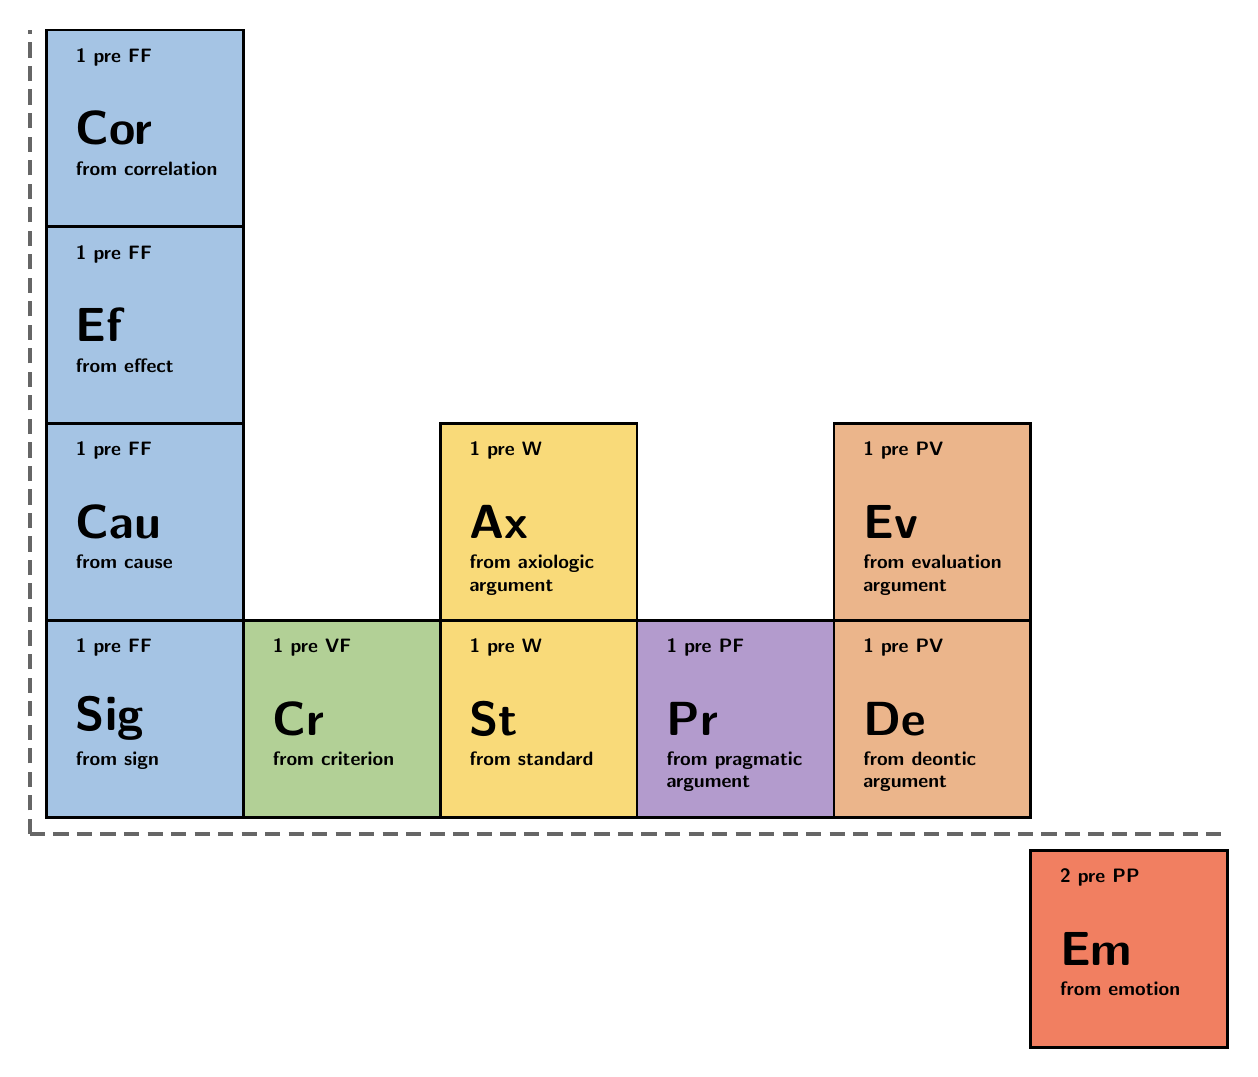
\begin{tikzpicture}[
        font=\sffamily
    ]
    %Defining a drawing structure
    \def\Arg[#1][#2][#3](#4)(#5){%1:Node name and label 2:description 3:type 4:position relative using positioning 5:color
        \node[
            line width=1pt,
            draw,
            #4,
            fill=#5,
            rectangle,
            inner sep=0,
            outer sep=0,
            minimum size=2.5cm
        ](#1){};
        \draw[every node/.append style={anchor=west}]
            (#1.center)++(-1,0) node {\LARGE\bfseries #1}
            (#1.center)++(-1,0.9) node {\scriptsize\bfseries #3}
            (#1.center)++(-1,-0.3) node[anchor= north west,align=left,font=\scriptsize\bfseries\sffamily]{ #2};
        }

    %Start drawing the thing...
    \definecolor{mycyan}{HTML}{A5C4E4}
    \definecolor{mygreen}{HTML}{B2D096}
    \definecolor{myyellow}{HTML}{F9DA79}
    \definecolor{mypurple}{HTML}{B39BCD}
    \definecolor{myorange}{HTML}{EBB58B}

    \Arg[Cor][from correlation][1 pre FF]()(mycyan)
    \Arg[Ef][from effect][1 pre FF](below=0 of Cor)(mycyan)
    \Arg[Cau][from cause][1 pre FF](below=0 of Ef)(mycyan)
    \Arg[Sig][from sign][1 pre FF](below=0 of Cau)(mycyan)
    \Arg[Cr][from criterion][1 pre VF](right=0 of Sig)(mygreen)
    \Arg[St][from standard][1 pre W](right=0 of Cr)(myyellow)
    \Arg[Ax][from axiologic \\ argument][1 pre W](above=0 of St)(myyellow)
    \Arg[Pr][from pragmatic \\ argument][1 pre PF](right=0 of St)(mypurple)
    \Arg[De][from deontic \\ argument][1 pre PV](right=0 of Pr)(myorange)
    \Arg[Ev][from evaluation \\ argument][1 pre PV](above=0 of De)(myorange)
    %Fron the other quadrant-
    \Arg[Em][from emotion][2 pre PP](below right=12pt and 0 of De)(myorange!70!red)

    \draw[dash pattern=on 5.5pt off 3pt,ultra thick,black!60]
        (De.south east) ++(2.5cm,-6pt) coordinate (axisX)
        (Cor.north west) ++ (-6pt,0) coordinate (axisY)
        (axisX -| axisY) edge (axisX) edge (axisY); % Using edges to obtain corner with dash line on.

    \end{tikzpicture}
\end{document}
